\documentclass[fleqn, a4paper. 12pt]{ltjsarticle} % lualatex guidance.tex
\usepackage{amsmath,txfonts}
\usepackage{amssymb}
\usepackage{url}
\usepackage[margin=31mm]{geometry}
\usepackage{graphicx}
\usepackage{color}
\usepackage{listings}
%ここからソースコードの表示に関する設定
\lstset{
  basicstyle={\linespread{0.6}},
  identifierstyle={\small},
  keywordstyle={\small\bfseries},
  ndkeywordstyle={\small},
  stringstyle={\small\ttfamily},
  frame={tb},
  breaklines=true,
  columns=[l]{fullflexible},
%  numbers=left,
  xrightmargin=1em,
  xleftmargin=2em,
  numberstyle={\scriptsize},
  stepnumber=1,
  numbersep=1em
}
\newcommand{\XA}[1]{\begingroup \color{red}}
\newcommand{\AX}[1]{\endgroup}
\lstnewenvironment{cppcode}
{\lstset{language=C++,
         basicstyle=\small\ttfamily,
         frame=single,
         breaklines=true,
         numbers=left}}
{}


\geometry{left=25mm,right=25mm,top=25mm,bottom=30mm}

\title{
2023年度 システムプログラミング実験\\
確率プログラミング\\
レポート}
\author{
学修番号: 22140003 \\
氏名: 佐倉仙汰郎 \\
}
\begin{document}
\date{
第1回レポート提出日:yyyy/mm/dd \\
第2回レポート提出日:yyyy/mm/dd \\
第3回レポート提出日:yyyy/mm/dd \\
}
\maketitle

\section*{はじめに}
本書ではシステムプログラミング実験第三回の課題を実験した結果を報告する.課題は乱数の生成、また乱数を用いた確率の解析である.解析結果をグラフと数値により示し、その結果について考察を行う.
\subsection*{実験の概要}

本実験ではモンテカルロ法を用いて解析を進める.
モンテカルロ法では乱数を用いてシミュレーションを行う手法のことである.
課題1ではモンテカルロシミュレーションを行うために必要な乱数の生成を行う関数をつくる.
課題2では課題1で作った関数を用いて、コイン投げのシミュレーションを行う.
課題3では課題1で作った関数を用いて、さいころ投げのシミュレーションを行う.
追加課題Aでは、課題1で作った関数を用いて、さいころ投げの趣味レーションを課題3とは違う設定で行う.
それぞれの課題で得られた結果をもとに考察を行う.

\subsection*{実験環境}
前節で説明した方法をC++言語\footnote{\url{https://isocpp.org/std/the-standard}}により実装した.実験環境の仕様を次に示す.
\begin{itemize}
    \item Central Processing Unit: 11th Gen Intel(R) Core(TM) i7-1167G7 @ 2.80 GHz
    \item 主記憶: Double Data Rate 4 Synchronous Dynamic Random-Access Memory
    \item コンパイラ: g++ version 11.2.0
    \item Operating System: Arch Linux\footnote{\url{https://archlinux.org/}}
    \item 数値型: 倍精度浮動小数点数\footnote{\url{https://www.gnu.org/software/gsl/doc/html/ieee754.html}}
  \end{itemize}
\newpage
\section*{課題1-1}
\section*{実験の説明}
区間 [0, 1) の一様乱数を独立に n 個生成する関数を作成する.作成した関数を用いて $n = 1000$ 個の乱数を生成し,その平均値と分散を計算する.
今回は標準ライブラリに搭載されている、std::random内の関数 std::random device, std::mt19937 および std::uniform real distributionを使用した。(ファイルkadai\_1\_1\_sentaro\_sakura.cppを参照)
\section*{実験結果}

メルセンヌツイスター法を用いて1000個の乱数から、平均値と分散を求めた結果が以下のとおりである.\\
$平均値: 0.498$\\
$分散: 0.0858$\\
平均値はおおよそ理論値に近くなった.分散が$0.0858$と非常に小さな値になっていることから一様に乱数が分布していることが分かる.
\section*{考察}
今回の実験で得られた値は理想地に近い値となった.このことからメルセンヌツイスター法が乱数の生成に妥当である.
\newpage
\section*{課題1-2}
\section*{実験の説明}
課題 1-1 で作成したプログラムをもとにコイン投げのシミュレーションプログラムを作成する.
作成したプログラムを用いて 1,000 回のコイン投げのシミュレーションを行い,表・裏それぞれが
出た確率を求める.ただし, 表が出る確率を $p$, 裏が出る確率を $1 − p$ とする.
レポートには,$p = 0.2, 0.5, 0.7$ の 3 通りそれぞれについて,関数 rnd exp を用いて生成した
$n =1,000$個のコイン投げに対する結果から考察を行う.シミュレーションで得られたコイ
ンの表・裏の確率は,有効数字 3 桁で報告する.\\
生成した $n$ 個の乱数 $r_1, . . . , r_n$ を用いて,$i$ 回目のコイン投げ試行の結果を以下のように定
める:$(i) r_i <= p $であれば,i 回目のコイン投げ試行で表が出たとする.$(ii) r_i > p $であれば,
$i$ 回目のコイン投げ試行で裏が出たとする.
\section*{実験結果}
\begin{equation}
  $p = 0.3$の時$0.704$\\
  $p = 0.5$の時$0.499$\\
  $p = 0.7$の時$0.282$\\
\end{equation}
実験結果は以上の通りになった.すべての$p$の値に対して理論値に近い値である.このことから、乱数生成が適切に稼働していることが分かった.
\newpage
\section*{課題1-3}
\section*{実験の説明}
サイコロ投げのシミュレーションプログラムを作成する.各目の出る確率は等確率とする.
作成したプログラムを用いて $1000$ 回の試行を行い,$1000$ 回の試行で出たサイコロの目の平
均値を求め,その結果を用いて,横軸を試行回数 $n$,縦軸を$n$ 回の試行の平均値とした
グラフを作成し、結果を考察する.
\section*{実験結果}
\begin{figure}[tb]
  \centering
  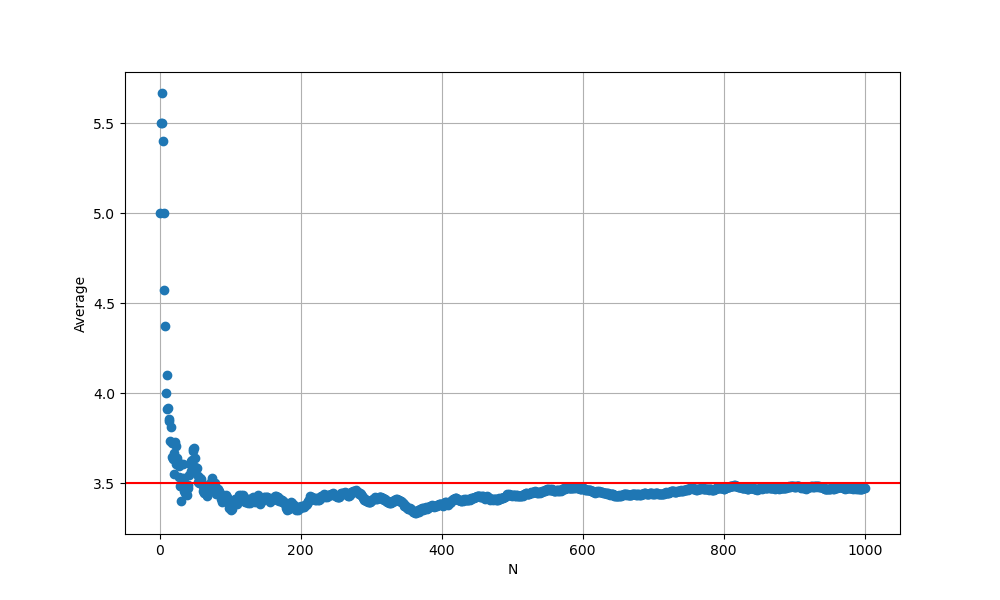
\includegraphics[width=\textwidth]{my_plot1-3.png}
  \label{f1}
  \caption{実験結果のグラフは、課題1-1で作った関数を参照}
\end{figure}
さいころの目を確率変数$X$とし、確率変数の期待値を$E[]$とする.さいころの期待値は以下の式で表せる.
\begin{align*}
  E[X] &= \frac{{1+2+3+4+5+6}}{6} \\[8pt]
  &= \frac{21}{6} \\[8pt]
  &= \frac{7}{2} \\[8pt]
  &= 3.5
  \label{e1}
\end{align*}
\begin{equation}
  平均値:3.53
\end{equation}
$1000$回さいころの目をふった平均値は図(1)の通りになる.
平均値が$n$の値が大きくになるにつれ$3.5$にちかずいていることがわかり、今回の実験で妥当な値が出ている.
\newpage
\section*{課題1-A}
\section*{実験の説明}
課題1-3 において各目 $i=1,2,...,1000  $の出る確率 $p_i$ が次のように偏っていたとする.$p_1 = p_3 =
p_5 = 1/9, p_2 = p_4 = p_6 = 2/9$. このとき,課題1-3 の結果がどう変わるかをグラフを作成して示し、その結果から考察を行う.
\section*{実験結果}
各目の出る確率が $p_1 = p_3 = p_5 = 1/9$ および $p_2 = p_4 = p_6 = 2/9$ の場合、各目が出る確率 $P(i)$ は以下のように表される.
\begin{equation}
  P(1) = P(3) = P(5) = \frac{1}{9}\\
  P(2) = P(4) = P(6) = \frac{2}{9}
\end{equation}
期待値$E$を計算するには以下のようになる.
\begin{align*}
  E &= \sum_{i=1}^{6} i \cdot P(i) \\[8pt]
  &= 1 \cdot \left(\frac{1}{9}\right) + 2 \cdot \left(\frac{2}{9}\right) + 3 \cdot \left(\frac{1}{9}\right) + 4 \cdot \left(\frac{2}{9}\right) + 5 \cdot \left(\frac{1}{9}\right) + 6 \cdot \left(\frac{2}{9}\right) \\[8pt]
  &= \frac{1}{9} + \frac{4}{9} + \frac{3}{9} + \frac{8}{9} + \frac{5}{9} + \frac{12}{9} \\[8pt]
  &= \frac{1 + 4 + 3 + 8 + 5 + 12}{9} \\[8pt]
  &= \frac{11}{3} \\[8pt]
  &= 3.67
\end{align*}
実験で得られた値は以下のとおりである.
\begin{equation}
  平均値:3.67
\end{equation}
となり、有効数値三桁では十分な精度である.
また図(2)からも理論値に知数いていることが分かる.
\begin{figure}[tb]
  \centering
  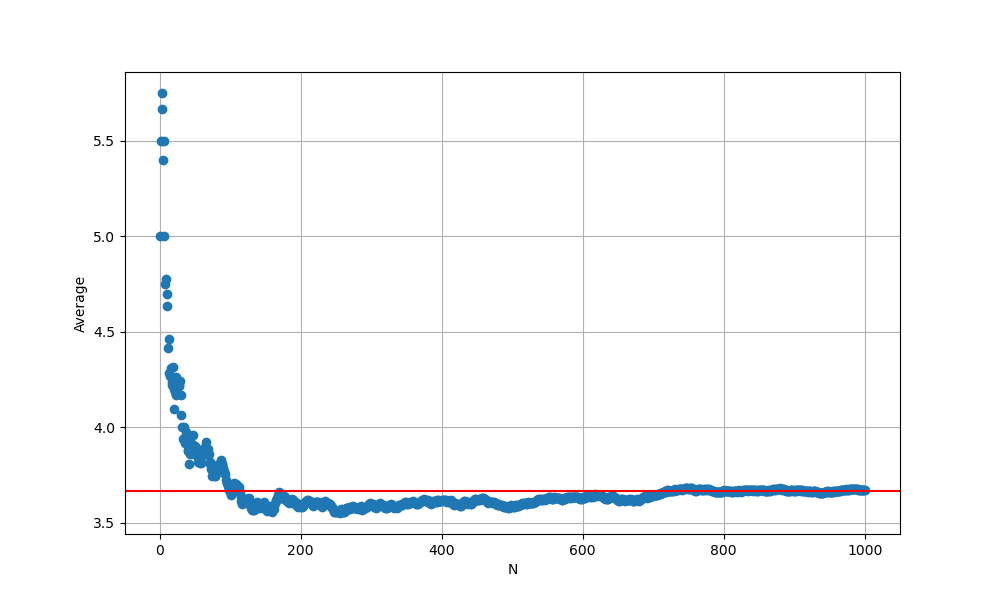
\includegraphics[width=\textwidth]{my_plot1-A.png}
  \label{f2}
  \caption{}
\end{figure}
\section*{おわりに}
今回の実験ではたくさんのソースコードを作り、様々なライブラリなどを制作した.課題の目標であった、実践的なコーディング能力上昇に大きく貢献したと思う.
課題が複数ある慣れない形式ではあったが、それぞれについて適切な考察を行えたと思う.
\newpage
\bibliography{reference}
\bibliographystyle{junsrt} 

\newpage
\section*{付録}
今回の課題に使用したソースコードを以下に示す.
\begin{cppcode}
  #include<iostream>
#include<random>
using namespace std;

//ランド関数を作る
void rnd_exp(double A[], int n){
    random_device rd;
    mt19937 gen(rd());
    uniform_real_distribution<double> distribution(0.0,1.0);
    for(int i = 0; i < n; i++){
        double r = distribution(gen);
        A[i] = r;
    }
}
int main(){
    int n = 1000;
    double A[n];
    rnd_exp(A,n);
    double sum1 = 0;
    double sum2 = 0;
    for(int i = 0; i < n ; i++){
        sum1 += A[i];
        sum2 += A[i] * A[i];
    }
    double ave = sum1 / n;
    cout << "平均値: " << sum1/n << endl;
    cout << "分散: " << sum2/n - ave*ave << endl;
    return 0;
}
\end{cppcode}
\begin{cppcode}
  #include<iostream>
#include<random>
using namespace std;

//ランド関数を作る
void rnd_exp(double A[], int n){
    random_device rd;
    mt19937 gen(rd());
    uniform_real_distribution<double> distribution(0.0,1.0);
    for(int i = 0; i < n; i++){
        double r = distribution(gen);
        A[i] = r;
    }
}

int main(){
    int n = 1000;
    double A[n];
    rnd_exp(A,n);
    double p1 = 0.3;
    double p2 = 0.5;
    double p3 = 0.7;
    double R1, R2, R3;
    R1 = 0;
    R2 = 0;
    R3 = 0;
    for(int i = 0; i < n; i++){
        if(A[i] < p1){
        }
        else if(p1 <= A[i] && A[i] <= p2 ){
            R1++;
        }
        else if(p2 < A[i] && A[i] <= p3){
            R1++;
            R2++;
        }
        else if(p3 < A[i]){
            R1++;
            R2++;
            R3++;
        }
    }
    cout << "p = 0.3の時" << R1/n << endl;
    cout << "p = 0.5の時" << R2/n << endl;
    cout << "p = 0.7の時" << R3/n << endl;

    return 0;
}
\end{cppcode}
\begin{cppcode}
  #include<iostream>
#include<random>
#include<fstream>
using namespace std;

//ランド関数を作る
void rnd_exp(double A[], int n){
    random_device rd;
    mt19937 gen(rd());
    uniform_real_distribution<double> distribution(0.0,1.0);
    for(int i = 0; i < n; i++){
        double r = distribution(gen);
        A[i] = r;
    }
}
int GenDice(){
    random_device rd;
    mt19937 gen(rd());
    uniform_int_distribution<int> distribution(1, 6);
    return distribution(gen);
}

int main(){
    ofstream of("DiceAverage.csv");
    of << "N,Average" <<endl; 
    int n = 1000;
    double A[n];
    rnd_exp(A,n);
    double sum = 0;

    for(int i = 0; i < n; i++){
        sum += GenDice();
        of << i+1 << "," << sum/(i+1) << endl;
    }
    cout << sum/n << endl;
    return 0;
}
\end{cppcode}
\begin{cppcode}
  #include<iostream>
#include<random>
#include<fstream>
using namespace std;

//ランド関数を作る
void rnd_exp(double A[], int n){
    random_device rd;
    mt19937 gen(rd());
    uniform_real_distribution<double> distribution(0.0,1.0);
    for(int i = 0; i < n; i++){
        double r = distribution(gen);
        A[i] = r;
    }
}
int GenDice(){
    random_device rd;
    mt19937 gen(rd());
    uniform_int_distribution<int> distribution(1, 9);
    int a = distribution(gen);
    if(a == 7) a = 2;
    if(a == 8) a = 4;
    if(a == 9) a = 6;
    return a;
}

int main(){
    ofstream of("DiceAverage1-A.csv");
    of << "N,Average" <<endl; 
    int n = 1000;
    double A[n];
    rnd_exp(A,n);
    double sum = 0;

    for(int i = 0; i < n; i++){
        sum += GenDice();
        of << i+1 << "," << sum/(i+1) << endl;
    }
    return 0;
}
\end{cppcode}
\newpage
\bibliography{reference}
\bibliographystyle{junsrt} 

(参考文献.\cite{example} などを参考に,bib ファイルの使い方はウェブなどで勉強すること.)

\end{document}